\documentclass{cours}
\usetikzlibrary{fit}
\usepackage[version=3]{mhchem}
\usepackage{etoolbox}
\usepackage{chemfig}
\usepackage{pgfplots}
\setcounter{chapter}{7}
\begin{document}

\chapter{Structure et propriétés des entités chimiques}

\section{Structure des atomes}%
\label{sec:structure_des_atomes}

\subsection{Constitution de l'atome}%
\label{sub:constitution_de_l_atome}
\begin{itemize}
	\item L'atome est constitué d'un ensemble d'\textbf{électrons} qui
	      \textit{gravitent} autour d'un \textbf{noyau}.
	\item Les \textbf{électrons} sont des particules fondamentales chargées
	      négativement ($q_e=-e=\SI{1.6e-19}{C}$) et dont la masse est
	      $m_e=\SI{9.1e-31}{kg}$.
	\item Le \textbf{noyau} est composé de protons et de neutrons très proches les
	      uns des autres.
	      \begin{itemize}
		      \item Un \textbf{proton} a une masse $m_P=\SI{1.6e-27}{kg}$ ($\simeq 2000 m_e$)
		            et une charge opposée à celle de l'électron $q_P=e=\SI{1.6e-19}{C}$
		      \item Un \textbf{neutron} a une masse \emph{presque} (à \si{e-3} près)
		            identique à celle du proton ($m_N\simeq m_P$) et a une charge électrique nulle
		            $q_N=0$.
	      \end{itemize}
	\item Un atome est \textbf{électriquement neutre}, c'est à dire que sa charge
	      électrique est nulle. Donc un atome contient autant de protons que d'électrons.
\end{itemize}

\subsection{Ordres de grandeur}%
\label{sub:ordres_de_grandeur}

\begin{itemize}
	\item Le proton est environ 2000 fois plus lourd que l'électron. plus de
	      \SI{99.9}{\percent} de la masse de l'atome est dans le noyau.

	\item La taille d'un atome d'hydrogène est d'environ \SI{25}{pm}
	      (\SI{25e-12}{m}), la taille de son noyau est d'environ \SI{0.8}{fm}
	      (\SI{0.8e-15}{m}) soit environ 30000 fois plus petit !
\end{itemize}
\subsection{Configuration électronique}%
\label{sub:configuration_electronique}

Les électrons d'un atome ne peuvent pas être décrits par la mécanique classique, il faut faire appel à la mécanique quantique. On peut montrer que l'état d'un électron autour d'un atome est caractérisé par 4 \textit{nombres quantiques} :

\begin{itemize}
	\item \textbf{$n$ : nombre quantique principal} : Caractérise l'énergie $E_n$
	      de l'électron
	      \begin{equation*}
		      E_n = \frac{\SI{-13.6}{eV}}{n^2} \quad \text{avec} \quad n\in\mathbb{N}
	      \end{equation*}
	      Il existe plusieurs fonctions d'onde d'énergie $E_n$, on dit que ce niveau
	      d'énergie est \emph{dégénéré}

	      Le nombre $n$ définit une \textbf{couche électronique}

	\item \textbf{$l$ : nombre quantique secondaire} : Caractérise la norme du
	      moment cinétique de l'électron autour du noyau.
	      \begin{equation*}
		      0 \leq l  \leq n-1
	      \end{equation*}
	      Le nombre $l$ définit une \textbf{sous-couche électronique}

	      On utilise une notation alphabétique pour les différentes valeurs de $l$ :

	      \begin{center}
		      \begin{tabular}{lllllll}
			      \toprule
			      $l$     & 0 & 1 & 2 & 3 & 4 & 5 \\
			      %\midrule
			      symbole & $s$ & $p$ & $d$ & $f$ & $g$ & $h$ \\
			      \bottomrule
		      \end{tabular}
	      \end{center}

	\item \textbf{$m_l$ : nombre quantique magnétique} : Caractérise la
	      projection du moment cinétique de l'électron sur l'axe $z$.
	      \begin{equation*}
		      -l \leq m_l \leq l
	      \end{equation*}


	      Le triplet de nombres $(n,l,m_l)$ définit une \textbf{orbitale atomique}, on
	      note la fonction d'onde associée $\Psi_{n, l, m_l}$.

	\item \textbf{$m_s$ : nombre quantique de spin} : Caractérise la projection
	      du moment cinétique intrinsèque de l'électron (il \og tourne \fg sur lui-même)
	      sur l'axe $z$.
	      \begin{equation*}
		      m_s = \pm \frac{1}{2}
	      \end{equation*}
\end{itemize}

Dans un atome, il est impossible que deux électrons aient leurs 4 nombres quantiques identiques (principe d'exclusion de Pauli). Chaque orbitale peut donc accueillir que 2 électrons, et sur une sous-couche de nombre quantique $l$ il peut y avoir au maximum 
\begin{eqencadre}
  N_l = 4l+2 \quad \text{électrons}
\end{eqencadre}

\begin{center}
  \begin{tabular}{@{}lllll@{}}
    \toprule
    Sous-couche & $s$ & $p$ & $d$ & $f$  \\
    \midrule
    Nombre d'électrons & 2 & 6 & 10 & 14 \\
    \bottomrule
  \end{tabular}
\end{center} 

En général, on cherche la structure électronique de l'état fondamental de l'atome, c'est à dire la structure de son état de plus basse énergie. Pour cela on utilisera la règle de Klechkowski :

\begin{loi}{Règle de Klechkowski}
  L'énergie d'une sous-couche est d'autant plus grande que $n+l$ est grand, et pour deux valeurs identiques de $n+l$ l'énergie est d'autant plus grande que $n$ est grand.

  Cette règle donne l'ordre de remplissage des sous-couches suivant :
  
  \begin{minipage}{0.5\linewidth}
  \begin{center}
    \def\lookup#1{\directlua {
    local array={"s","p","d","f"}; tex.print(array[#1])}}
    
    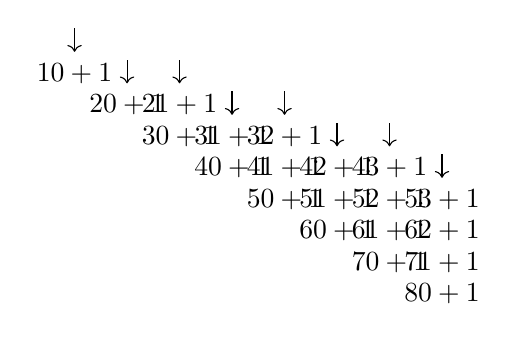
\begin{tikzpicture}
      \foreach \n in {1,...,8}{
        \pgfmathsetmacro{\lf}{\n-1}
        \foreach \l in {0,...,\lf}{
           \newbool{draw}
           \pgfmathparse{ifthenelse(\n+\l<9,"true", "false")}
           \setbool{draw}{\pgfmathresult}
           \ifbool{draw}{\draw ({(\n+\l)/1.5}, -\n/2.5) node[anchor=mid]{$\n\lookup{\l+1}$};}{}
        }      
      }
      \draw[<-] (1/1.5,-1/2.5+0.3) -- ++(0, 0.3);
      \draw[<-] (2/1.5,-2/2.5+0.3) -- ++(0, 0.3);
      \draw[<-] (3/1.5,-2/2.5+0.3) -- ++(0, 0.3);
      \draw[<-] (4/1.5,-3/2.5+0.3) -- ++(0, 0.3);
      \draw[<-] (5/1.5,-3/2.5+0.3) -- ++(0, 0.3);
      \draw[<-] (6/1.5,-4/2.5+0.3) -- ++(0, 0.3);
      \draw[<-] (7/1.5,-4/2.5+0.3) -- ++(0, 0.3);
      \draw[<-] (8/1.5,-5/2.5+0.3) -- ++(0, 0.3);
    \end{tikzpicture}
  \end{center}
\end{minipage}%
  \begin{minipage}{0.5\linewidth}
    Ordre de remplissage :

    $1s\,2s\,2p\,3s\,3p\,4s\,3d\,4p\, 5s\, 4d\,  \ldots$ 
\end{minipage}%
\end{loi}


	      \textbf{Exemples :} \begin{itemize}
		      \item $\ce{[^12_6C]} = 1s^22s^22p^2$
		      \item $\ce{[_8O]} = 1s^22s^22p^4$
	      \end{itemize}

Les électrons responsables de la réactivité chimique de l'atome sont les
électrons des sous-couche externes, ceux dont l'énergie est la plus élevée.

\emph{Les électrons de valence} sont les électrons de nombre quantique
\textbf{$n$ le plus élevé} ainsi que les électrons des sous-couches
\textbf{partiellement remplies}. Les autres électrons sont les \emph{électrons
	de c\oe{}ur}.

\textbf{Exemples :}
\begin{itemize}
  \item L'oxygène $\ce{[^{16}_8O]} = \underbrace{1s^2\vphantom{p}}_\text{c\oe{}ur\vphantom{\text{l}}} \underbrace{2s^22p^4}_\text{valence}$

  \item Le fer $\ce{[_{26}Fe]} = \underbrace{1s^22s^22p^63s^23p^6}_\text{c\oe{}ur\vphantom{\text{l}}} \underbrace{4s^23d^6\vphantom{p}}_\text{valence}$
\end{itemize}

\textbf{Remarque : } La configuration électronique des électrons de c\oe{}ur est toujours celle d'un gaz noble (dernière colonne de la classification périodique). On peut simplifier l'écriture de la configuration électronique :
 $[\ce{_{26}Fe}] = [\ce{Ar}]4s^23d^6$
\section{Structue des molécules}%
\label{sec:structue_des_molecules}

\subsection{Modèle de la liaison covalente}%
\label{sub:modele_de_la_liaison_covalente}

L'interaction attractive à l'origine d'une liaison covalente est produite par la mise en commun d'électrons qui sont partagés par les atomes participant à la liaison. Seuls les électrons de valence peuvent participer à une liaison covalente.
\begin{center}
  \begin{tikzpicture}
    %tikz chimie
    \draw[fill=gray!20] (0,0) circle (0.5) node(A) {A};
    \draw[fill=gray!20] (3,0) circle (0.4) node(B) {B};
    \draw ($(A)+(-70:1)$) arc(290:70:1) .. controls (1.5, 0.5) .. ($(B)+(110:1)$) arc(110:-110:1) .. controls(1.5, -0.5) .. ($(A)+(-70:1)$);
    \draw[fill=gray] (0, 1) circle(0.1) (3, -1) circle(0.1) coordinate (ev);
    \draw[<-] ($(ev)+(-45:0.15)$) -- ++(1, -0.5) node[right, align=left]{électrons de valence\\(orbitale moléculaire)};
    \draw (A) circle (0.6);
    \draw (A) circle (0.75);
    \draw[fill=gray] (A) ++ (30:0.75) circle(0.1);
    \draw[fill=gray] (A) ++ (-80:0.75) circle(0.1);
    \draw (B) circle (0.5);
    \draw (B) circle (0.65);
    \draw[fill=gray] (B) ++ (120:0.65) circle(0.1);
    \draw[fill=gray] (B) ++ (-40:0.65) circle(0.1) coordinate (ec);
    \draw[<-] ($(ec)+(0.15, 0)$) -- ++(1, 0) node[right, align=left]{électrons de c\oe{}ur\\(orbitale atomique)};
  \end{tikzpicture}
\end{center}


Les électrons de valence sont \emph{délocalisés} sur les deux atomes liés. Dans le \emph{modèle de la liaison covalente localisée}, on considère que les électrons de liaison sont \emph{localisés} sur l'axe A--B. On symbolise la liaison par \chemfig{A-B}.

La longueur d'une liaison covalente est de l'ordre de \SI{100}{pm}. L'énergie nécessaire à briser une liaison covalente, appelée \emph{énergie de liaison} est de l'ordre de 100 à \SI{1000}{kJ\per\mol} (énergie nécessaire pour briser une mole de liaisons) ou de 1 à \SI{10}{eV} par liaison.


\subsection{Représentation de Lewis des molécules}%
\label{sub:representation_de_lewis_des_molecules}

L'expérience montre que les ions monoatomiques les plus stables possèdent la même configuration électronique que celle d'un gaz noble (qui possède 8 électrons de valence)

\begin{loi}{Règle de l'octet}
Lorsqu'ils forment une molécule, les atomes forment des liaisons covalentes pour s'entourer de 8 électrons de valence.
\end{loi}

Par exemple, deux atomes de chlore~ \chemfig{\charge{0=., 90=\|, 180=\|, -90=\|}{Cl}}~ partagent leur électron célibataire pour former une liaison covalente :

\begin{center}
  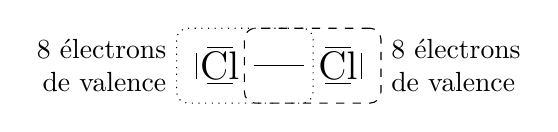
\begin{tikzpicture}
    \draw (0,0) node[inner sep=5pt] (Cl1) {\Large\chemfig{\charge{90=\|, 180=\|, -90=\|}{Cl}}};
  \draw (1.5,0) node[inner sep=5pt] (Cl2) {\Large\chemfig{\charge{0=\|, 90=\|, -90=\|}{Cl}}};
    \draw (Cl1) -- (Cl2);
    \node[fit=(Cl1) (Cl2.west), draw, rounded corners, dotted](rect1){};
    \draw (rect1.west) node[left, align=right]{8 électrons\\de valence};
    \node[fit=(Cl1.east) (Cl2), draw, rounded corners, dashed](rect2){};
    \draw (rect2.east) node[right, align=left]{8 électrons\\de valence};
    %\draw (Cl1.west) to[out=90, in=180] (Cl1.north) to[out=0, in=90] ($(Cl2.west)+(0.1, 0)$);
  \end{tikzpicture}
\end{center}

Les atomes doivent parfois former plusieurs liaisons covalentes pour satisfaire la règle de l'octet. Par exemple dans la molécule de dioxygène :

\begin{center}
  \begin{tikzpicture}
  \draw (0,0) node[inner sep=5pt] (O1) {\Large\chemfig{\charge{135=\|, 225=\|}{O}}};
\draw (1.5,0) node[inner sep=5pt] (O2) {\Large\chemfig{\charge{45=\|, -45=\|}{O}}};
    \draw ($(O1.east)+(0,1pt)$) -- ($(O2.west)+(0,1pt)$);
    \draw ($(O1.east)+(0,-1pt)$) -- ($(O2.west)+(0,-1pt)$);
    \node[fit=(O1) (O2.west), draw, rounded corners, dotted](rect1){};
    \draw (rect1.west) node[left, align=right]{8 électrons\\de valence};
    \node[fit=(O1.east) (O2), draw, rounded corners, dashed](rect2){};
    \draw (rect2.east) node[right, align=left]{8 électrons\\de valence};
    %\draw (Cl1.west) to[out=90, in=180] (Cl1.north) to[out=0, in=90] ($(Cl2.west)+(0.1, 0)$);
  \end{tikzpicture}
\end{center}


\begin{loi}{Règle du duet}
Les atomes qui comportent très peu d'électrons (\ce{H}, \ce{He}, \ce{Li}) ont tendance à s'entourer de 2 électrons de valence (comme l'hélium)
\end{loi}

Par exemple pour la molécule de dihydrogène : \chemfig{H-H}.

Pour un ion polyatomique, la règle est la même, il faut en plus déterminer où sont situées les charges.

Par exemple la représentation de Lewis de l'ion hydroxyde (\ce{HO-}) est :
\begin{center}
  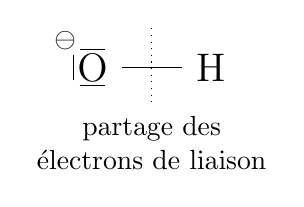
\begin{tikzpicture}
    
  \draw (0,0) node[inner sep=5pt] (O) {\Large\chemfig{\chemabove{\charge{90=\|, 180=\|, -90=\|}{ O}}{{\hspace{-7mm}\scriptstyle \ominus}}}};
    \draw (1.5,0) node[inner sep=5pt] (H) {\Large\chemfig{H}};
    \draw (O) -- (H);
    \draw[dotted](0.75, 0.5) -- (0.75,-0.5) node[below, align=center]{partage des\\électrons de liaison};
  \end{tikzpicture}
\end{center}
En séparant les électrons de liaison entre les deux atomes, on remarque que l'oxygène est entouré de 7 électrons de valence alors qu'il n'en possède naturellement que 6. Il porte donc une charge négative.


Les règles de l'octet et du duet fonctionnent bien pour les atomes des deux premières lignes de la classification périodique. Le soufre (S) et le phosphore (P) peuvent être hypervalents, tout comme les métaux de transition (bloc~d) ainsi que les éléments du bloc~f. 

Par exemple la représentation de Lewis de l'acide sulfurique \ce{H2SO4} est :
\begin{center}
  \chemfig{
  H-
  \charge{90=\|, -90=\|}{O}-
  S(=[::90]\charge{45=\|, 135=\|}{O})(=[::-90]\Charge{-135=\|, -45=\|}{O})-
  \Charge{90=\|, -90=\|}{O}-
  H
  }
\end{center}

\subsubsection{Méthode de détermination de la représentation de Lewis}%
\label{ssub:méthode_de_détermination_de_la_représentation_de_lewis}

\begin{center}
\begin{tabular}{@{}p{8cm}p{8cm}@{}}
\toprule
Méthode générale & Exemple pour l'ion \ce{CO3^{2-}}\\
\midrule
1 -- Déterminer le nombre de doublets à placer en calculant le nombre total d'électrons de valence. & $n_v(\ce{C}) = 4$ ; $n_v(\ce{O})=6$. Le nombre total d'électrons à placer est $n_e=4+6\times3+2 = 24$ soit 12 doublets.  \\[1cm]

2 -- Établir la structure de la molécule, on privilégie une configuration en étoile avec un atome central et des atome périphériques (pas de cycles). &  On place \ce{C} au centre. On obtient la structure : 

\vspace{1em}
\parbox{8cm}{\centering\chemfig{O-C(-[::60]O)-[::-30]O}} \\[1cm]

3 -- Ajouter les doublets restants en respectant la règle de l'octet ou du duet. & 
 Il reste 9 doublets à ajouter.

 \vspace{1em}
 \parbox{8cm}{\centering\chemfig{\charge{135=\|, 225=\|}{O}=C(-[::60]\charge{60=\|, 150=\|, -30=\|}{O})-[::-30]\charge{60=\|, -120=\|, -30=\|}{O}} }\\[1cm]

 4 -- Calculer les charges formelles portées par chaque atome & ~

\vspace{1em}
 \parbox{8cm}{\centering
 \chemfig{\charge{135=\|, -135=\|}{O}=C(-[::60]\chemabove{\charge{60=\|, 150=\|, -30=\|}{O}}{\scriptstyle\hspace{5mm}\ominus})-[::-30]\chemabove{\charge{60=\|, -120=\|, -30=\|}{O}}{\scriptstyle\hspace{5mm}\ominus}}} \vspace{1em} \\[1cm]

\bottomrule
\end{tabular}
\end{center}
 
La règle de l'octet ne peut pas toujours être satisfaite, par exemple pour la molécule de dioxyde d'azote \ce{NO2} :
\begin{center}
\chemfig{\chemabove{\charge{90=\|, 180=\|, -90=\|}{O}}{\scriptstyle\hspace{-7mm}\ominus} - \chembelow{\charge{90=\.}{N}}{\scriptstyle\oplus} = \charge{45=\|, -45=\|}{O}}
\end{center}
L'atome d'azote est entouré de 7 électrons de valence. Le molécules qui ne respectent pas la règle de l'octet sont généralement instables et très réactives.
\section{Géométrie et polarité des molécules}%
\label{sec:geometrie_et_polarite_des_molecules}

\subsection{Électronégativité}%
\label{sub:electronegativite}

L'électronégativité $\chi$ d'un élément chimique est un nombre sans dimension qui quantifie sa capacité à capter des électrons (les siens ou ceux des autres). Plus un élément est électronégatif, plus il est capable d'attirer vers lui des électrons.

Un atome très électronégatif sera qualifié d'\emph{oxydant} car il pourra capter les électrons d'autres atomes.

Un atome très peu électronégatif est qualifié de \emph{réducteur} car il cédera facilement un ou plusieurs électrons à d'autres atomes.

L'électronégativité augmente de gauche à droite et diminue du haut vers le bas de la classification périodique.

Les métaux alcalins (colonne 1) sont très réducteurs, leur électronégativité est faible et les halogènes (colonne 17) sont très oxydants, leur électronégativité est élevée.

\subsection{Polarité des liaisons et des molécules}%
\label{sub:polarite_des_liaisons_et_des_molecules}

Les électrons de liaison ne sont pas forcément distribués équitablement sur les deux atomes liés. L'atome le plus électronégatif attirera plus les électrons vers lui.
\begin{itemize}
  \item Si les électronégativités des deux atomes sont similaires, les électrons de liaison sont distribués symétriquement sur les deux atomes.
  \begin{center}
    \begin{tikzpicture}
      \draw (0,0) node[draw, circle, inner sep=0.2cm, fill=gray!20] {H};
      \draw (2,0) coordinate (B) node[draw, circle, inner sep=0.2cm, fill=gray!20] {H};
      \draw (-70:1) arc (290:70:1) .. controls (1,0.5) .. ($(B)+(110:1)$) arc (110:-110:1) .. controls (1,-0.5) .. (-70:1);
    \draw[fill=gray] (B) ++ (90:1) circle(0.1);
    \draw[fill=gray] (A) ++ (-170:1) circle(0.1);
    \begin{scope}[xshift=7cm]
      \draw (0,0) node[draw, circle, inner sep=0.2cm, fill=gray!20] (H1) {H};
      \draw (2,0) node[draw, circle, inner sep=0.2cm, fill=gray!20] (H2) {H};
      \draw (H1) -- (H2);
    \end{scope}
    \end{tikzpicture}
  \end{center}

  \item Si l'atome A est nettement plus électronégatif que l'atome B, il attirera plus les électrons de liaison. Il y aura une charge négative $-\delta$  autour de l'atome A et une charge positive $+\delta$  autour de l'atome B, on dit que la liaison est \emph{polarisée}. Dans ces conditions, la liaison possède un \emph{moment dipolaire} $\vec \mu = \delta \oa{AB}$. 

\begin{center}
    \begin{tikzpicture}
      \draw (0,0) node[draw, circle, inner sep=0.2cm, fill=gray!20] {O};
      \draw (2,0) coordinate (B) node[draw, circle, inner sep=0.2cm, fill=gray!20] {H};
      \draw (-70:1.3) arc (290:70:1.3) .. controls (1.2,0.8) .. ($(B)+(110:0.8)$) arc (110:-110:0.8) .. controls (1.2,-0.8) .. (-70:1.3);
    \draw[fill=gray] (A) ++ (90:1.3) circle(0.1);
    \draw[fill=gray] (A) ++ (200:1.3) circle(0.1);
    \begin{scope}[xshift=7cm]
      \draw (0,0) node[draw, circle, inner sep=0.2cm, fill=gray!20] (O) {O};
      \draw (2,0) node[draw, circle, inner sep=0.2cm, fill=gray!20] (H) {H};
      \draw (O) -- (H);

      \draw (O.north) node[above]{$-\delta$ };
      \draw (H.north) node[above]{$+\delta$ };
      \draw[latex-latex] ($(O.south)+(0, -0.1)$) -- ($(H.south)+(0, -0.1)$) node[midway, fill=white, inner sep=2pt] {$d$} ;
      \draw[-latex] ($(O.south)+(0, -0.6)$) -- ($(H.south)+(0, -0.6)$) node[midway, below] {$\vec \mu$} ;
    \end{scope}
    \end{tikzpicture}
  \end{center}
\end{itemize}

Une liaison covalente peut posséder un moment dipolaire, il en va de même pour une molécule dans son ensemble. Le moment dipolaire d'une molécule est égal à la somme \emph{vectorielle} des moments dipolaires des liaisons qui la constituent. La polarité d'une molécule dépend de la polarité des liaisons qui la composent mais aussi de la \emph{géométrie} de la molécule.

Une molécule adopte la géométrie qui lui permet de minimiser sont énergie. Tout comme un ressort tend à minimiser son énergie potentielle élastique.

Par exemple la liaison \ce{C-O} est polaire car l'oxygène est plus électronégative que le carbone, mais la molécule de \ce{CO2} ne possède pas de moment dipolaire permanent car les moments dipolaires des liaison sont alignés et s'annulent.
\begin{center}
  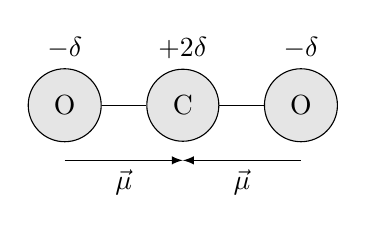
\begin{tikzpicture}
    \draw (0,0) node[circle, fill=gray!20, inner sep=2mm, draw](O1){O};
    \draw (1.5,0) node[circle, fill=gray!20, inner sep=2mm, draw](C){C};
    \draw (3,0) node[circle, fill=gray!20, inner sep=2mm, draw](O2){O};
    \draw (O1.north) node[above] {$-\delta$}; 
    \draw (O2.north) node[above] {$-\delta$}; 
    \draw (C.north) node[above] {$+2\delta$}; 
    \draw (O1) -- (C) -- (O2);
    \draw[-latex] (0, -0.7) -- (1.5, -0.7) node[below, midway]{$\vec \mu$}; 
    \draw[-latex] (3, -0.7) -- (1.5, -0.7) node[below, midway]{$\vec \mu$}; 
  \end{tikzpicture}
\end{center}


Par contre la molécule d'eau possède un moment dipolaire à cause de sa géométrie non rectiligne :

\begin{center}
  \begin{tikzpicture}
    \draw (0,0) node[circle, fill=gray!20, inner sep=2mm, draw](O){O};
    \draw (-150:2) node[circle, fill=gray!20, inner sep=2mm, draw](H1){H};
    \draw (-30:2) node[circle, fill=gray!20, inner sep=2mm, draw](H2){H};
    \draw[->] ($(O)+(-0.6, 0)$) -- ++(210:1) node[midway, above left]{$\vec \mu$} ;
    \draw[->] ($(O)+(0.6, 0)$) -- ++(-30:1) node[midway, above right]{$\vec \mu$} ;
    \draw[->] ($(O)+(0, -0.6)$) -- ++(-90:0.8) node[midway, right]{$\vec \mu_\text{tot}$} ;
    \draw (H1) -- (O) -- (H2);
    \draw (O.north) node[above]{$-2\delta$};
    \draw (H1.west) node[left]{$+\delta$};
    \draw (H2.east) node[right]{$+\delta$};
    %\draw[-latex] (0, -0.7) -- (1.5, -0.7) node[below, midway]{$\vec \mu$}; 
    %\draw[-latex] (3, -0.7) -- (1.5, -0.7) node[below, midway]{$\vec \mu$}; 
  \end{tikzpicture}
\end{center}
Le moment dipolaire d'une molécule d'eau est de $|\vec \mu_\text{tot}|\approx\SI{6e-30}{\coulomb\meter}$ 

Le moment dipolaire d'une molécule est habituellement donné en \textit{Debye} (D) avec $\SI{1}{D} \approx \SI{3.34e-30}{\coulomb\meter} $ 

\section{Interactions entre les entités chimiques}%
\label{sec:interactions_entre_les_entites_chimiques}


La cohésion des différentes molécules pour former des phases condensées (liquide ou solide) est assurée par des \emph{forces intermoléculaires}. Ces forces étant beaucoup plus faibles que les liaisons covalentes, on parles de \emph{liaisons faibles}.

\subsubsection{Interactions de Van der Waals}%
\label{ssub:interactions_de_van_der_waals}
Les forces entre les moments dipolaires des molécules sont appelées \emph{forces de Van der Waals}. On distingue plusieurs types de forces en fonction des dipôles qui interagissent.

\begin{itemize}
  \item \textbf{Les forces de Keesom} correspondent à l'interaction électrostatique entre les dipôles permanents des molécules. Elles n'existent qu'entre des molécules polaires. Plus les moments dipolaires des molécules sont importants, plus les forces de Keesom le sont.
  \begin{center}
    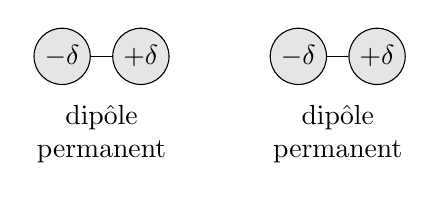
\begin{tikzpicture}
      \draw (0,0) node[circle, draw, inner sep=2pt, fill=gray!20] (moins){$-\delta$}; 
      \draw (1,0) node[circle, draw, inner sep=2pt, fill=gray!20] (plus){$+\delta$};
      \draw (moins) -- (plus);

      \draw (0.5, -0.5) node[below, align=center]{dipôle\\permanent};
      \draw (3.5, -0.5) node[below, align=center]{dipôle\\permanent};

      \draw (3,0) node[circle, draw, inner sep=2pt, fill=gray!20] (moins){$-\delta$}; 
      \draw (4,0) node[circle, draw, inner sep=2pt, fill=gray!20] (plus){$+\delta$};
      \draw (moins) -- (plus);
      
    \end{tikzpicture}
  \end{center}

  \item \textbf{Les forces de Debye} sont dues à l'interaction entre un dipôle permanent et un dipôle induit. Un dipôle induit est un moment dipolaire qui apparait dans une molécule lorsqu'on l'approche d'une molécule polaire.

  \begin{center}
    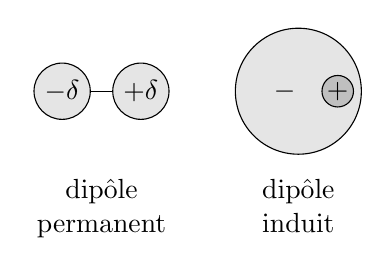
\begin{tikzpicture}
      \draw (0,0) node[circle, draw, inner sep=2pt, fill=gray!20] (moins){$-\delta$}; 
      \draw (1,0) node[circle, draw, inner sep=2pt, fill=gray!20] (plus){$+\delta$};
      \draw (moins) -- (plus);
      
      \draw[fill=gray!20] (3,0) circle(0.8cm) node[xshift=-5]{$-$};
      \draw[fill=gray!50] (3.5,0) circle(0.2cm) node{$+$};

      \draw (0.5, -1) node[below, align=center] {dipôle\\permanent};
      \draw (3, -1) node[below, align=center] {dipôle\\induit};
    \end{tikzpicture}
  \end{center}
  Elles sont d'autant plus fortes que les molécules sont polarisables. Les molécules les plus polarisables sont celles qui contiennent des \emph{gros} atomes qui comportent beaucoup d'électrons.

  \item \textbf{Les forces de London} sont prépondérantes lorsque les molécules ne possèdent pas de dipôle permanent. Dans ce cas elles peuvent présenter un moment dipolaire instantané du aux fluctuation de la distribution de leurs électrons. Ces moments dipolaires instantanés peuvent induire un moment dipolaire dans les molécules voisines.
  \begin{center}
    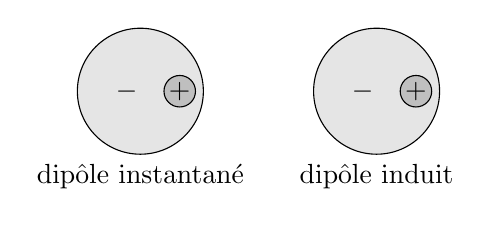
\begin{tikzpicture}
      \draw[fill=gray!20] (3,0) circle(0.8cm) node[xshift=-5]{$-$};
      \draw (3, -0.8) node[below] {dipôle induit};
      \draw[fill=gray!50] (3.5,0) circle(0.2cm) node{$+$};

      \draw[fill=gray!20] (0,0) circle(0.8cm) node[xshift=-5]{$-$};
      \draw (0, -0.8) node[below] {dipôle instantané};
      \draw[fill=gray!50] (0.5,0) circle(0.2cm) node{$+$};
    \end{tikzpicture}
  \end{center}

  Elles sont d'autant plus intenses que les molécules sont polarisables.
\end{itemize}


Les liaisons de Van Der Waals ont une énergie de l'ordre de 1 à \SI{10}{kJ\per\mol} et une longueur de l'ordre de \SI{500}{pm}

\subsubsection{Liaison hydrogène}%
\label{ssub:liaison_hydrogene}

L'interaction intermoléculaire la plus forte apparait lorsqu'un atome d'hydrogène s'intercale entre deux atomes très électronégatifs (\ce{O}, \ce{F}, \ce{N}). On symbolise cette liaison par 
\begin{equation*}
  \ce{X-H \cdots Y}
\end{equation*}
où \ce{X} et \ce{Y} sont les atomes électronégatifs.

La liaison \ce{X-H} est très polaire et l'hydrogène porte une charge positive importante. Cette charge positive va alors attirer le doublet non liant de \ce{Y} pour former la liaison.

Cette liaison possède aussi un caractère covalent (délocalisation des électrons de \ce{X} et \ce{Y}). 

L'intensité et la longueur de la liaison est intermédiaire entre liaison covalente et interaction de Van Der Walls, l'énergie de liaison est de l'ordre de \SI{20}{\kilo\joule\per\mol}. Elle est responsable des températures élevées de changement d'état de l'eau.

Les molécules peuvent former des liaisons hydrogène intra-moléculaires. C'est par exemple le cas de la molécule d'ADN dont les deux brins de la double hélice sont liés pas des liaisons hydrogène. Les liaisons hydrogène intramoléculaires peuvent empêcher la formation de liaisons hydrogène inter moléculaires. On peut citer l'exemple de l'acide maléique et de l'acide fumarique. L'acide maléique forme des liaisons hydrogène intra-moléculaires qui empèche la formation de liaisons hydrogène intermoléculaires. Alors que l'acide fumarique ne contient pas de liaison hydrogène intramoléculaire, ce qui lui permet de former des liaisons hydrogène intermoléculaire et possède donc une température de fusion bien plus élevée ($T_\text{fus} = \SI{130}{\celsius}$ pour l'acide maléique et $T_\text{fus}=\SI{226}{\celsius}$ pour l'acide fumarique.)
\begin{center}
  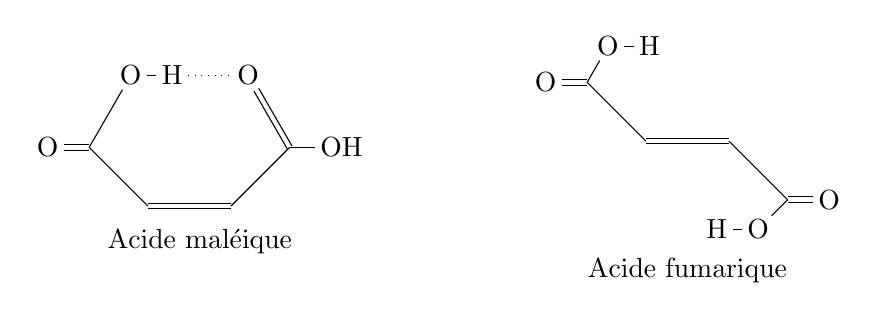
\begin{tikzpicture}
    \draw (0,0) node[](A){\chemfig{O=[,0.5](-[::60]O-[,0.5]H?)-[7]=-[1](=[:120]O?[,,dotted])-[,0.5]OH}};
    \draw (A.south) node[below] {Acide maléique};
    \draw (A.east) ++ (4,0) node(B)[]{\chemfig{O=[,0.5](-[::60,0.5]O-[,0.5]H)-[7]=-[7](=[,0.5]O)-[5,0.5]O-[4,0.5]H}};
    \draw (B.south) node[below] {Acide fumarique};
\end{tikzpicture}
\end{center}

\subsubsection{Températures de changement d'état}%

La force des interactions entre les molécules d'un corps condensé (solide ou liquide) est directement reliée aux températures de changement d'état du corps en question. Plus les interactions sont intenses, plus les températures de changement d'état sont élevées.

 \begin{center}
  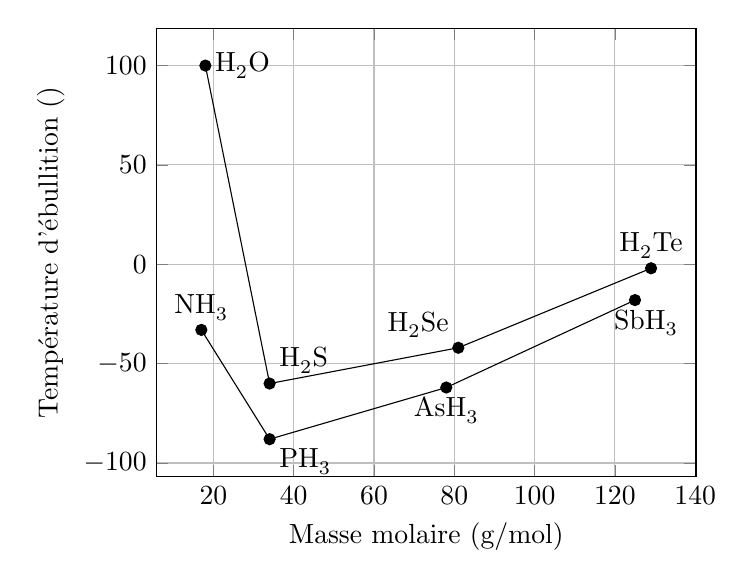
\begin{tikzpicture}
    %tikz chimie
    \begin{axis}[
    xlabel=Masse molaire (\si{g/mol}),
    ylabel=Température d'ébullition (\si{\celsius}),
    grid=major,
    ]
      \addplot[mark=*,
         ] table[x=M, y=Teb]{
    compose         M      Teb    Tfus
    \ce{H20}         18    100      0 
    \ce{H2S}         34    -60    -85
    \ce{H2Se}        81    -42    -66
    \ce{H2Te}       129     -2    -49
      };
      \addplot[mark=*,
         ] table[x=M, y=Teb]{
    compose    M      Teb
    \ce{NH3}        17     -33
    \ce{PH3}       34     -88
    \ce{AsH3}       78     -62
    \ce{SbH3}       125    -18
      };
    \draw (axis cs:18, 100) node[right]{\ce{H2O}};
    \draw (axis cs:34, -60) node[above right]{\ce{H2S}};
    \draw (axis cs:81, -42) node[above left]{\ce{H2Se}};
    \draw (axis cs:129, -2) node[above]{\ce{H2Te}};

    \draw (axis cs:17, -33) node[above]{\ce{NH3}};
    \draw (axis cs:34, -88) node[below right]{\ce{PH3}};
    \draw (axis cs:78, -62) node[below]{\ce{AsH3}};
    \draw (axis cs:125, -18) node[below, xshift=4]{\ce{SbH3}};
    \end{axis}
  \end{tikzpicture}
  %\space{1cm}
  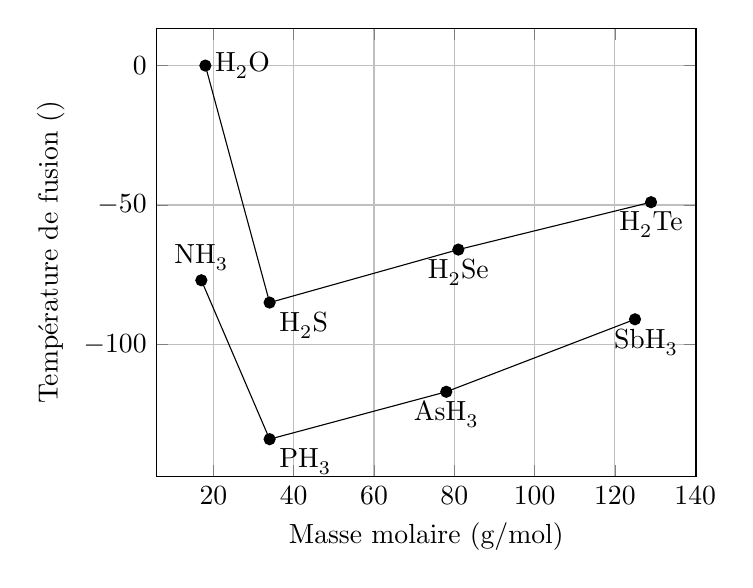
\begin{tikzpicture}
    \begin{axis}[
    xlabel=Masse molaire (\si{g/mol}),
    ylabel=Température de fusion (\si{\celsius}),
    grid=major,
    ]
      \addplot[mark=*,
         ] table[x=M, y=Tfus]{
    compose         M      Teb    Tfus
    \ce{H20}         18    100      0 
    \ce{H2S}         34    -60    -85
    \ce{H2Se}        81    -42    -66
    \ce{H2Te}       129     -2    -49
      };
      \addplot[mark=*,
         ] table[x=M, y=Tfus]{
    compose    M      Tfus
    \ce{NH3}        17     -77
    \ce{PH3}       34     -134
    \ce{AsH3}       78     -117
    \ce{SbH3}       125    -91
      };
    \draw (axis cs:18, 0) node[right]{\ce{H2O}};
    \draw (axis cs:34, -85) node[below right]{\ce{H2S}};
    \draw (axis cs:81, -66) node[below]{\ce{H2Se}};
    \draw (axis cs:129, -49) node[below]{\ce{H2Te}};

    \draw (axis cs:17, -77) node[above]{\ce{NH3}};
    \draw (axis cs:34, -134) node[below right]{\ce{PH3}};
    \draw (axis cs:78, -117) node[below]{\ce{AsH3}};
    \draw (axis cs:125, -91) node[below, xshift=4]{\ce{SbH3}};
    \end{axis}
  \end{tikzpicture}
  \captionof{figure}{Températures d'ébullition (à gauche) et de fusion (à droite) de différents composés hydrogénés en fonction de leur masse molaire.}
   \label{fig:temp_transition}
\end{center} 

Sur la figure~\ref{fig:temp_transition}, on trace les températures de changement d'état de certaines molécules hydrogénées. On remarque que pour les plupart des molécules, plus leur masse molaire est importante, plus la température de changement d'état est élevée. Ceci est dû au fait que plus l'atome (autre que l'hydrogène) qui compose la molécule est gros, plus il est polarisable et plus les interactions de Van der Waals seront importante. 

On remarque l'exception notable de l'eau (\ce{H2O)}) et de l'ammoniac (\ce{NH3}) dont les températures de changement d'état sont anormalement élevées. Ceci est causé par la présence de liaisons hydrogène entre les molécules qui sont beaucoup plus intenses que les liaisons de Van der Waals.



\section{Solubilité et miscibilité}%
\label{sec:solubilite_et_miscibilite}

Dans une solution, le solvant est l'espèce chimique largement majoritaire. Les autres espèces chimiques sont les solutés.

\subsubsection{Caractéristiques d'un solvant}%
\label{ssub:caracteristiques_d_un_solvant}
Un solvant peut posséder plusieurs caractéristiques qui influences fortement les réactions chimiques qui peuvent s'y dérouler
\begin{itemize}
  \item Le \textbf{pouvoir ionisant} du solvant est sa capacité à dissocier les liaisons ioniques des molécules qui y sont présentes. Plus le moment dipolaire des molécules du solvant est élevé, plus il est ionisant. 

  Exemples : L'eau est un solvant très ionisant, le cyclohexane (\ce{C6H12}) est apolaire et donc non ionisant.

  \item Le \textbf{pouvoir dissociant} d'un solvant est sa capacité à séparer les paires d'ions. Plus la permittivité relative $\epsilon_r$ d'un solvant est élevée, plus il est dissociant car il écrante plus efficacement les charges électriques.

  Exemple : L'eau est un solvant très dissociant ($\epsilon_r\approx 80$), le cyclohexahe l'est beaucoup moins ($\epsilon_r\approx 2$)  

  \item On dit qu'un solvant est \textbf{protique} (ou protogène) si ses molécules sont susceptibles d'établir des liaisons hydrogène avec les solutés.

  Exemple : l'eau est un solvant protique.
\end{itemize}

\subsubsection{Mise en solution d'espèces chimiques}%
\label{ssub:mise_en_solution_d_especes_chimiques}
Pour dissoudre un solide dans un solvant, il faut briser les liaisons qui existent entre les ions (solide ionique) ou les molécules qui composent le solide.

S'il s'agit d'un solide ionique, il faut que le solvant atténue les interactions entre ions (permittivité élevée) et qu'il existe une interaction attractive entre les molécules du solvant et les ions (moment dipolaire, liaisons hydrogène).

En ce qui concerne un solide moléculaire, il faut que les interactions de Van Der Waals entre les molécules du solvant soient plus intenses que celles qui existent entre les molécules du solide.  

La mise en solution d'un composé ionique se fait en plusieurs étapes :
\begin{itemize}
  \item ionisation : les liaisons ioniques sont brisées ;
  \item disssociation : l'anion et le cation sont séparés ;
  \item solvatation : les molécules du solvant forment des liaisons faibles avec les ions (Van Der Waals, hydrogène, ...)
\end{itemize}

\subsubsection{Miscibilité de solvants}%
\label{ssub:miscibilite_de_solvants}
Deux solvant A et B sont miscibles si l'intensité des interactions intermoléculaires  (A,A), (B,B) et (A,B) sont du même ordre de grandeur.

En général, les solvants miscibles ont des caractéristiques similaires : un solvant polaire protique sera miscible avec un autre solvant polaire protique (eau et éthanol) mais pas avec un solvant apolaire aprotique (eau et cyclohexane)








\end{document}
